\documentclass[compress]{beamer}

\usetheme{Hamburg}

\usepackage[T1]{fontenc}
\usepackage[utf8]{inputenc}

\usepackage{lmodern}

%\usepackage[english]{babel}
\usepackage[ngerman]{babel}

\usepackage{eurosym}
\usepackage{listings}
\usepackage{lstautogobble}
\usepackage{microtype}
\usepackage{textcomp}
\usepackage{siunitx}
\usepackage{csquotes}
\usepackage{graphicx}
\usepackage{xcolor}
\usepackage{tikz}
\usepackage{tabularx}
\usepackage{physics}
\usepackage{amsmath}
\usepackage{amsfonts}
\usepackage{amssymb}
\usepackage{mathtools}
\usepackage{todonotes}
\usepackage{xfrac}
\usepackage{multirow}
\usepackage{hyperref}
\usepackage[noabbrev]{cleveref}
\usetikzlibrary{calc,positioning,decorations.pathreplacing,calligraphy}
\usepackage{upquote}

\sisetup{%
    locale = DE,
    per-mode = symbol,
    range-phrase = \text{--},
    range-units = single,
    separate-uncertainty = true
}

\lstset{
    basicstyle=\ttfamily\footnotesize,
    frame=single,
    numbers=left,
    language=C,
    breaklines=true,
    breakatwhitespace=true,
    postbreak=\hbox{$\hookrightarrow$ },
    showstringspaces=false,
    autogobble=true,
    upquote=true,
    tabsize=4,
    captionpos=b,
    morekeywords={int8_t,uint8_t,int16_t,uint16_t,int32_t,uint32_t,int64_t,uint64_t,size_t,ssize_t,off_t,intptr_t,uintptr_t,mode_t}
}

\title{HowTo: Linux}
% \subtitle{Veranstaltung}
\author{Ruben 14felgenh, Hauke 14stieler}
%\institute{Arbeitsbereich Wissenschaftliches Rechnen\\Fachbereich Informatik\\Fakultät für Mathematik, Informatik und Naturwissenschaften\\Universität Hamburg}

\usepackage{datetime}
\newcommand{\datef}[3]{%
    \newdate{datex}{#1}{#2}{#3}
    \date{\protect\displaydate{datex}}
}
\let\oldthedate\thedate
\makeatletter
\makeatother
\datef{06}{12}{2022}

%\usepackage[style=numeric,bibencoding=utf8,backend=biber]{biblatex}
%\addbibresource{literature.bib}



\begin{document}

    \begin{frame}
        \titlepage
    \end{frame}

\section{Basics}

\begin{frame}{Terminal Historie}
    \begin{itemize}
        \item 19. Jahrhundert Drucker für Telegramme
        \item Später \textbf{T}ele\textbf{ty}pe-writer (TTY)
        \begin{itemize}
        	\item Gerät für Ein-/Ausgabe an Computern = Terminal
            \item Auch per Telefonkabel
            \item UNIX besaß TTY Treiber
        \end{itemize}
        \item Dumb Terminals (bis 1970er)
        \item Smart Terminals (ab Mitte 1960er)
        \item Virtuelle/Pseudo Terminals
        \begin{itemize}
        	\item \textbf{P}seudo-Tele\textbf{ty}pe -- PTY
        	\item ab Mitte 1990er
        	\item Terminal-Emulatoren (z.B. \texttt{konsole}, \texttt{xterm} oder \texttt{gnome-terminal}) verbinden sich mit PTY
        \end{itemize}
    \end{itemize}
\end{frame}


\begin{frame}{Historie}
	\begin{center}
		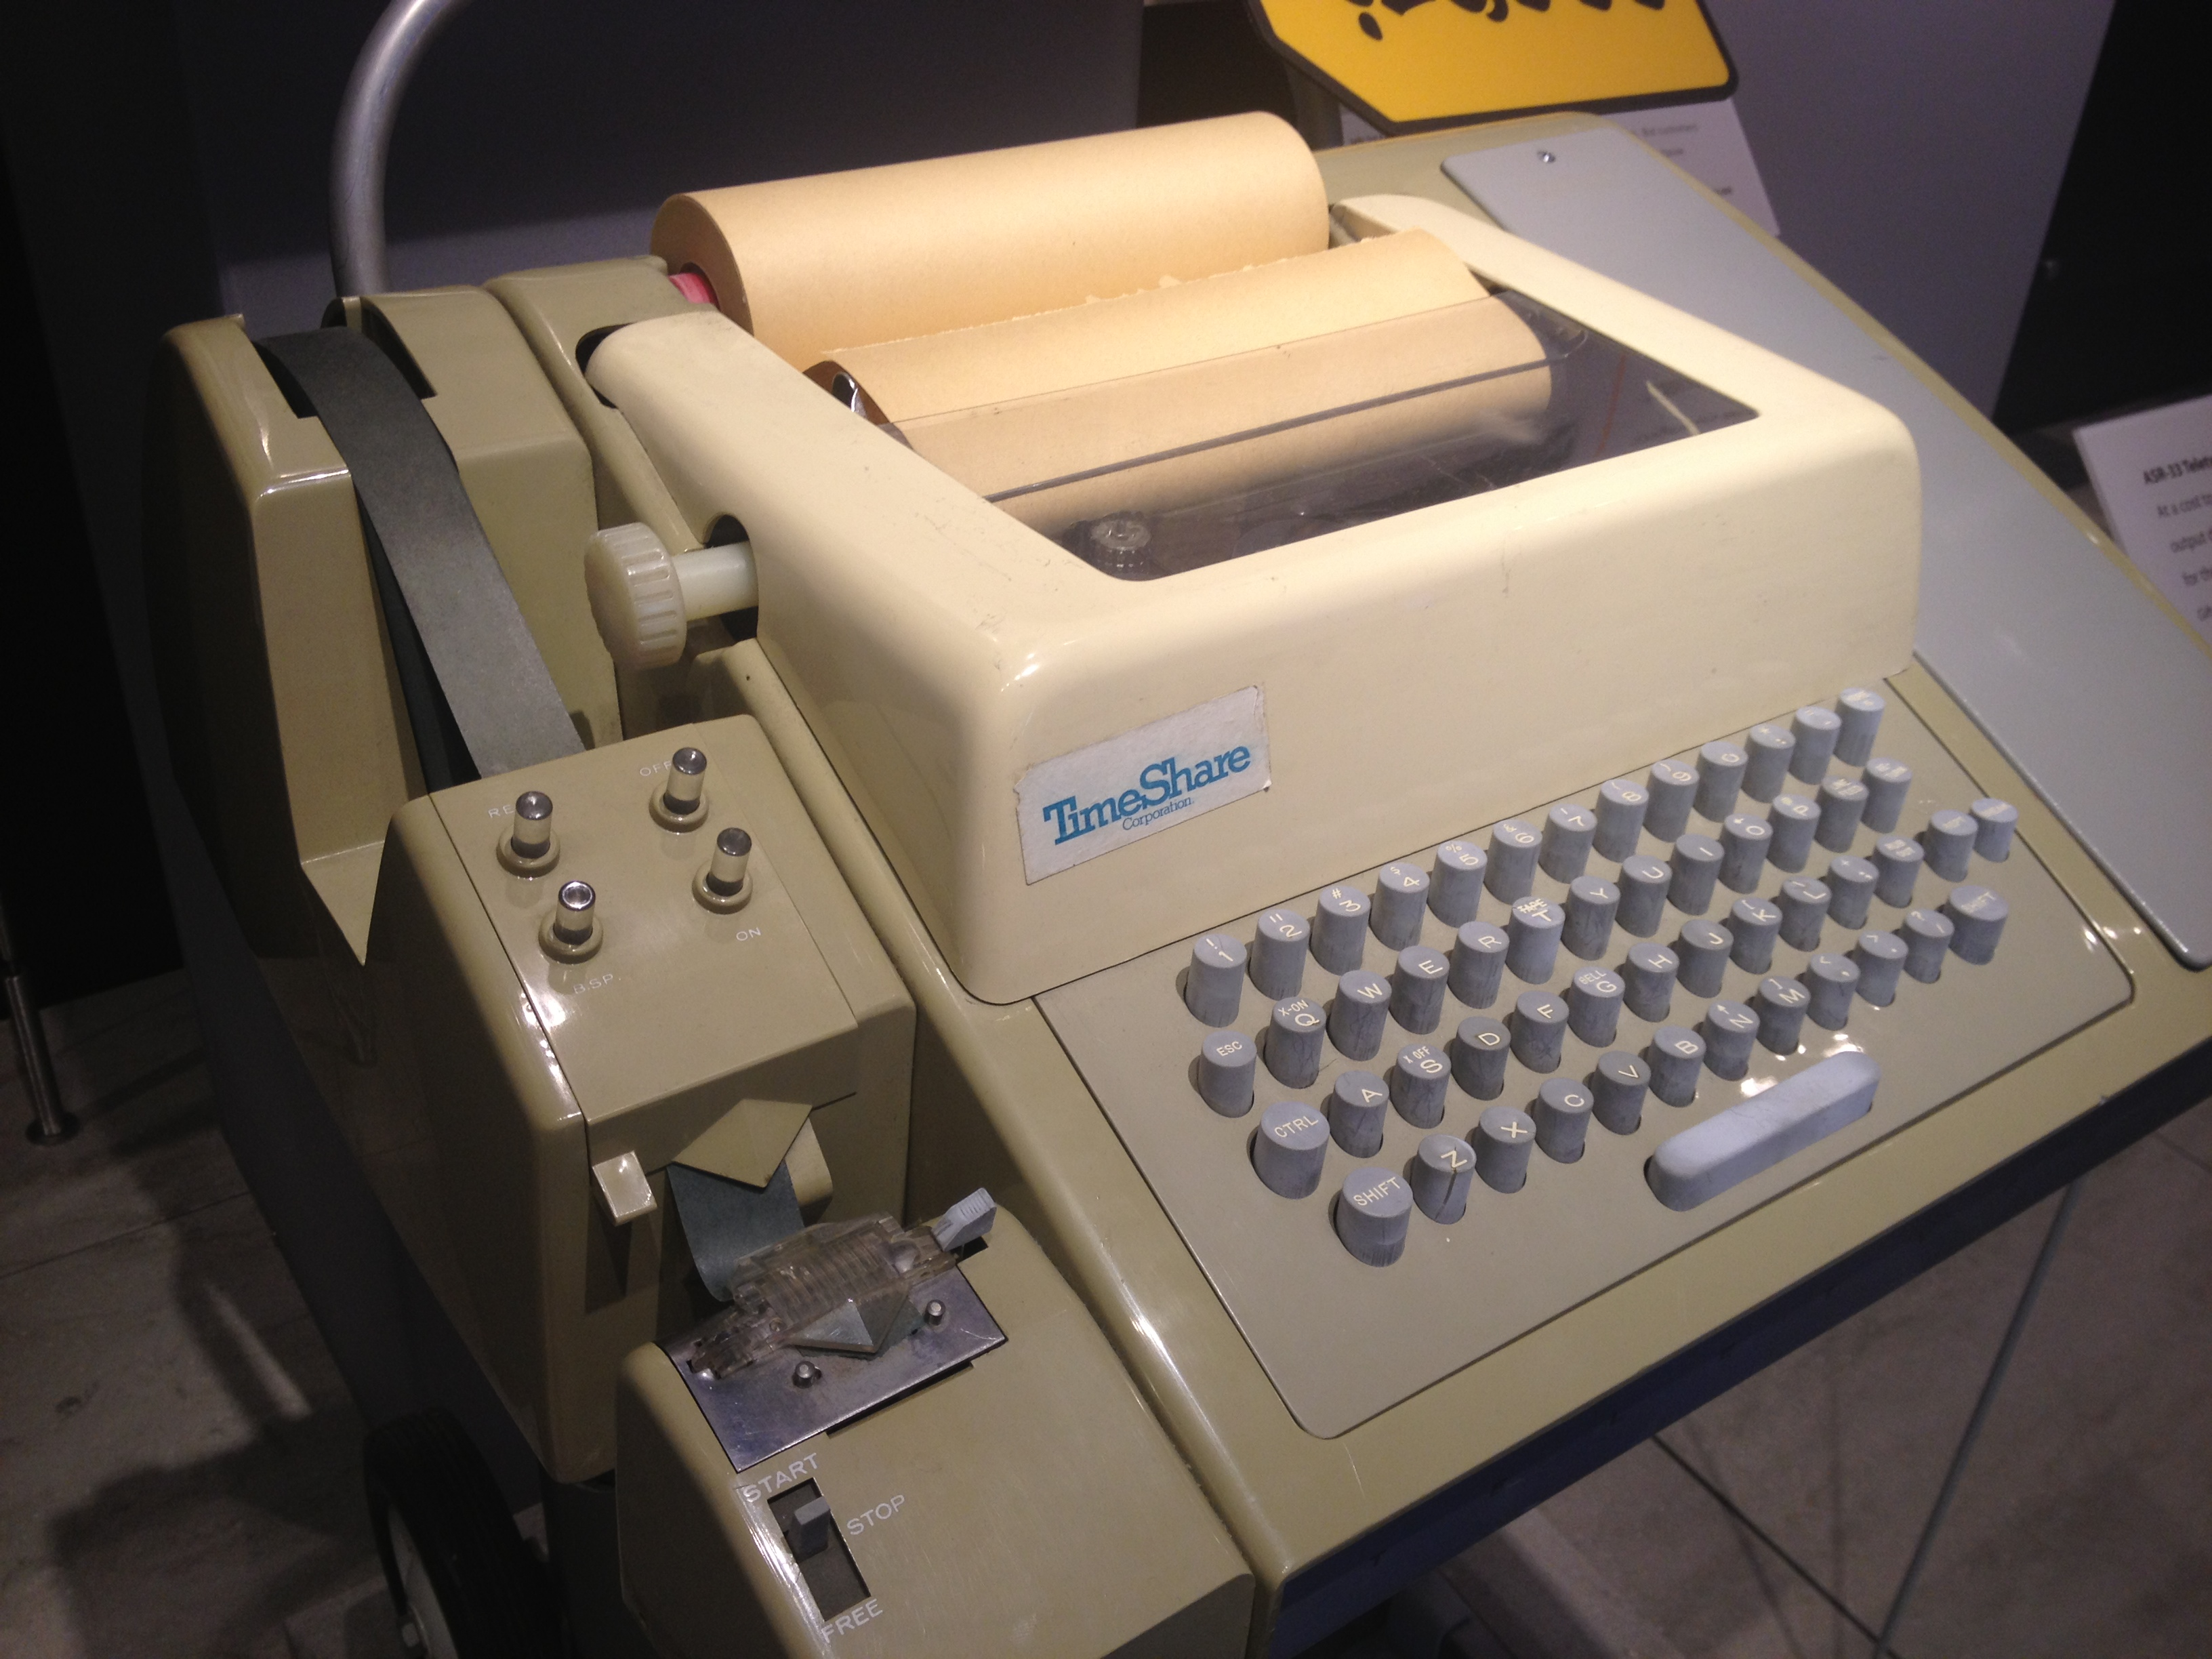
\includegraphics[height=0.7\textheight]{tty}
		\\
		Teletype ASR-33 (1963) mit Papierrolle als Ausgabe.
	\end{center}
\end{frame}

\begin{frame}{Historie}
	\begin{center}
		\only<1>{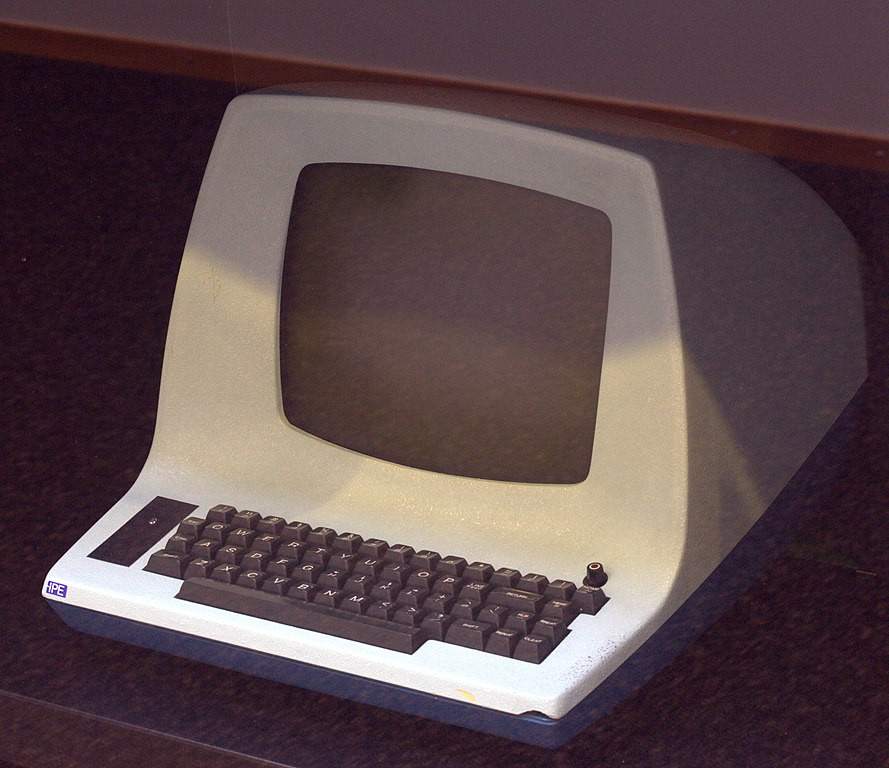
\includegraphics[height=0.7\textheight]{ADM-3A}}
		\only<2>{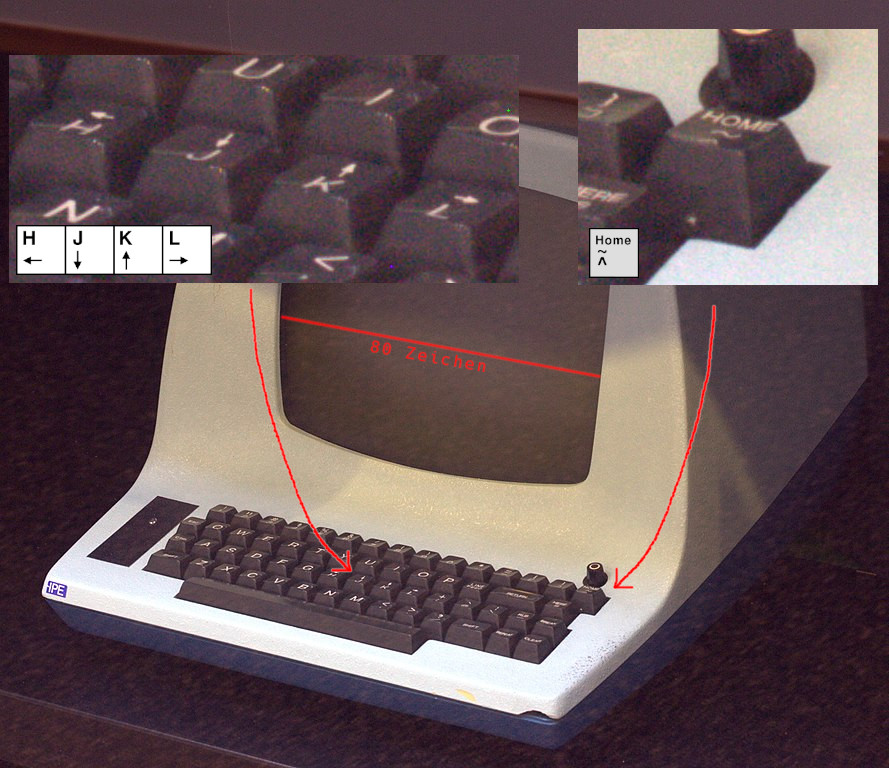
\includegraphics[height=0.7\textheight]{ADM-3A-zoomed-in}}
		\\
		\only<1-2>{Terminal ADM-3A (1976)}\visible<2>{: "`\raisebox{-0.77ex}{\~{}}"' (Tilde) auf "`Home"'-Taste, Pfeile auf H J K L Tasten \& 80 Zeichen pro Zeile.}
	\end{center}
\end{frame}


\begin{frame}[fragile]{Begriffe}
\begin{itemize}
    \item Kommandozeile / Konsole / CLI
    \item Shell
    \begin{itemize}
\item \verb+sh+
\item \verb+bash+
\item \verb+zsh+
\item \verb+ksh+
\item \verb+csh+
\item \verb+dash+
\item \verb+fish+
\end{itemize}
\item Terminal
\item Terminal-Emulator
\end{itemize}
\end{frame}

\begin{frame}[fragile]{Befehle}
\begin{itemize}
\item Shell-Built-Ins:
\begin{itemize}
\item \verb+pwd+
\item \verb+cd+
\item \verb+echo+
\item \verb+true+
\item \verb+false+
\item \verb+type+
\end{itemize}
\item Programme:
\begin{itemize}
\item \verb+firefox+
\item \verb+touch+
\item \verb+ls+
\item \verb+cat+
\item \verb+less+
\item \verb+man+
\end{itemize}
\end{itemize}
\end{frame}

\begin{frame}[fragile]{Argumente u.Ä.}
Es gibt Flags...
\begin{itemize}
\item \verb+firefox --help+
\item \verb+firefox -h+
\end{itemize}
... Parameter, ...
\begin{itemize}
\item \verb+type echo+
\item \verb+man echo+
\end{itemize}
... und Argumente.
\begin{itemize}
\item \verb+ls --color=always+
\item \verb+dd if=/dev/urandom count=1+
\end{itemize}
\end{frame}

\begin{frame}[fragile]{Ein- und Ausgaben}
\begin{itemize}
\item \verb+stdout+
\item \verb+stderr+
\item \verb+stdin+
\item Exit Codes
\item Ausgaben in Dateien umleiten:\\
\verb+echo foobar > foobar.txt+
\item Ausgaben als Eingaben für andere Programme verwenden: \\
\verb+echo foobar | rev+
\item Ausgaben in Variablen speichern:\\
\verb+meinname=$(whoami)+\\
\verb+echo $meinname+
\end{itemize}
\end{frame}

\begin{frame}[fragile]{History und Autovervollständigung}
\begin{itemize}
\item History:
\begin{itemize}
\item Pfeiltasten
\item \verb+history+
\item \verb+cat ~/.bash_history+
\item Strg + R
\end{itemize}
\item Autovervollständigung: Tab
\end{itemize}
\end{frame}

\section{Dateisystem}

\begin{frame}[fragile]{Dateien}
\begin{itemize}
\item Erstellen: \verb+touch foo.txt+
\item Lesen: \verb+cat foo.txt+ oder \verb+less foo.txt+
\item Schreiben:
\begin{itemize}
\item \verb+>+ überschreibt die Datei
\item \verb+>>+ hängt hinten an die Datei an.
\end{itemize}
\item Filtern: \verb+grep suchtext foo.text+
\item Kopieren: \verb+cp quelle.txt ziel.txt+
\item Umbenennen / Verschieben: \verb+mv vorher.txt nachher.txt+
\item Löschen: \verb+rm foo.txt+
\end{itemize}
\end{frame}

\begin{frame}[fragile]{Texteditoren}
    \begin{itemize}
        \item \verb+nano+
        \item \verb+micro+
        \item \verb+vi+ / \verb+vim+ / \verb+neovim+
        \item \verb+emacs+
    \end{itemize}
    \vspace{3mm}
    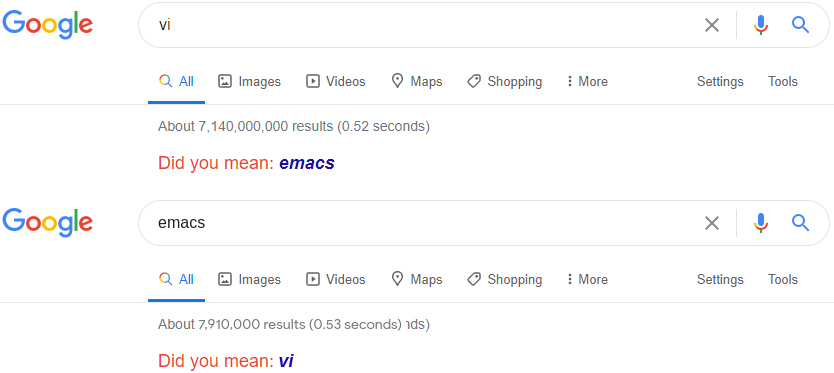
\includegraphics[width=.9\textwidth]{emacsvi.png}
\end{frame}

\begin{frame}[fragile]{Ordner}
\begin{itemize}
\item Erstellen: \verb+mkdir foo+
\item Inhalt auflisten: \verb+ls+
\item Kopieren: \verb+cp -r quelle ziel+
\item Umbenennen / Verschieben: \verb+mv vorher nachher+
\item Löschen: \verb+rm -r foo+
\end{itemize}
\end{frame}

\begin{frame}[fragile]{Dateien und Ordner suchen}
\begin{itemize}
\item Dateien suchen: \\
\verb+find -name foo.txt+ \\
\verb+find -name "*.txt*+ \\
\verb+find -type d -name bar+
\item Nach bestimmten Texten in Dateien suchen:\\
\verb+grep -Hirn 'suchtext'+
\end{itemize}
\end{frame}


\begin{frame}[fragile]{\texttt{ls} im Detail}
\begin{verbatim}
 $ ls -lahd .bashrc .local
 -rw-r--r-- 1 ruben ruben 3.5K Apr  4  2022 .bashrc
 drwx------ 5 ruben ruben 4.0K Oct 19 13:39 .local
\end{verbatim}

\hspace*{0.2mm}
\begin{tikzpicture}[scale=0.2]
\newcommand{\drawbrace}[3]{\draw [decorate,decoration={brace,mirror}] ($(#1-0.45,0)$) -- ($(#2+0.45,0)$) node[below=6mm,anchor=south,pos=0.5] {#3};}
\drawbrace{0}{10}{a}
\drawbrace{11}{12}{b}
\drawbrace{13}{18}{c}
\drawbrace{19}{24}{d}
\drawbrace{25}{29}{e}
\drawbrace{30}{42}{f}
\drawbrace{43}{50}{g}
\end{tikzpicture}
{
\setbeamertemplate{enumerate items}[default]
\begin{enumerate}[a)]
\item Berechtigungen
\item Anzahl Sub-Einträge
\item Besitzer
\item Besitzer-Gruppe
\item Größe
\item Zeit der letzten Änderung
\item Name
\end{enumerate}
}

\end{frame}

\begin{frame}[fragile]{Berechtigungen}
    \vspace{-8mm}

\Huge
\begin{verbatim}
 -rw-r--r-- 1 ruben ruben 3.5K Apr  4  2022 .bashrc
 drwx------ 5 ruben ruben 4.0K Oct 19 13:39 .local
\end{verbatim}

\normalsize

\hspace*{3mm}
\begin{tikzpicture}[scale=0.45]
    \newcommand{\drawbrace}[3]{\draw [decorate,decoration={brace,mirror}] ($(#1+0.05,0)$) -- ($(#2-0.05,0)$) node[below=6mm,anchor=south,pos=0.5] {#3};}
    \drawbrace{0}{1}{a}
    \drawbrace{1}{4}{b}
    \drawbrace{4}{7}{c}
    \drawbrace{7}{10}{d}
\end{tikzpicture}

{
    \setbeamertemplate{enumerate items}[default]
    \begin{enumerate}[a)]
        \item Ordner?
        \item Besitzer (\texttt{u})
        \item Besitzer-Gruppe (\texttt{g})
        \item Alle anderen (\texttt{o})
    \end{enumerate}
}

\vspace{-20mm}
\hspace*{65mm}
\begin{tabular}{|ll|}
\hline
\verb+d+:& Directory \\
\verb+r+:& Read \\
\verb+w+:& Write \\
\verb+x+:& Execute \\
\hline
\end{tabular}

\end{frame}

\begin{frame}[fragile]{Berechtigungen und Besitzer ändern}
\begin{itemize}
\item Datei für alle lesbar machen:\\
\verb|chmod a+r foo.txt|
\item Datei ausführbar machen:\\
\verb|chmod +x foo.txt|
\item Besitzer auf \enquote{hauke} ändern:\\
\verb+chown hauke:haukesgruppe foo.txt+
\end{itemize}
\end{frame}


\section{Netzwerk und Internet}

\begin{frame}[fragile]{SSH}
\begin{itemize}
\item Mit SSH können wir uns auf entfernten Rechnern einloggen:
\item \verb+ssh 4felgenh@rzssh1.informatik.uni-hamburg.de+
\item \url{https://mafiasi.de/SSH}
    \end{itemize}
\end{frame}

\begin{frame}[fragile]{Dateien herunterladen}
\begin{itemize}
\item \verb+curl example.org+
\item \verb+wget example.org+
\end{itemize}
\end{frame}

\section{Skripte}

\begin{frame}[fragile]{Shell-Skripte}
\verb+bash+ ist eine vollwertige Programmiersprache mit
\begin{itemize}
\item Variablen
\item Parametern
\item Verzweigung
\item Schleifen
\item Funktionen
\item Datenstrukturen
\begin{itemize}
\item Arrays
\item Maps
\end{itemize}
\end{itemize}
\end{frame}

\begin{frame}[fragile]{Mein erstes Shell-Skript}
\begin{verbatim}
#!/usr/bin/env bash

echo Hallo Welt
\end{verbatim}

\begin{itemize}
\item Skript ausführbar machen:\\
\verb|chmod +x meinskript.sh|
\item Skript ausführen:\\
\verb+./meinskript.sh+
\end{itemize}
\end{frame}

\begin{frame}[fragile]{Variablen}
\begin{verbatim}
#!/usr/bin/env bash

wer=Welt

echo Hallo $wer

wer=mafia

echo Hallo $wer
\end{verbatim}
\end{frame}

\begin{frame}[fragile]{Parameter}
\begin{verbatim}
#!/usr/bin/env bash

wer=$1

echo Hallo $wer
\end{verbatim}
\end{frame}

\begin{frame}[fragile]{Verzweigung}
\begin{verbatim}
#!/usr/bin/env bash

wer=$1

echo Hallo $wer

if [ "$wer" == "mafia" ] ; then
    food=Pizza
else
    food=Pasta
fi

echo Hier ist dein Teller $food
\end{verbatim}
\end{frame}

\begin{frame}[fragile]{Schleifen}
\begin{verbatim}
#!/usr/bin/env bash

echo Ich aß heute 5 Kekse. Erst den 1. Keks...

for i in {2..5} ; do
    echo Und dann den $i. Keks...
done
\end{verbatim}
\end{frame}

\begin{frame}[fragile]{Funktionen}
\begin{verbatim}
#!/usr/bin/env bash

function hallo (
    wer=$1
    echo Hallo $wer
)

bye() (
    wer=$1
    echo Bye $wer
)

hallo $1
bye $1
\end{verbatim}
\end{frame}

\begin{frame}[fragile]{Anführungszeichen und Klammern}
\vspace*{-2.5mm}
\footnotesize
\begin{itemize}
\item Strings:\\
\verb+name='Meine Textdatei.txt'+
\item Erhalten von Whitespace:\\
\verb+cat "$name"+
\item Command Substitution:\\
\verb+content="$(cat "$name")"+\\
\verb+content="`cat "$name"`"+
\item Compound Statements:\\
\verb+{echo foo ; echo bar}+\\
\verb+(echo foo ; echo bar)+
\item Test Brackets:\\
\verb+if [[ "$variable" == "foo" ]] ; then ...+
\verb+if [ "$variable" == "foo" ] ; then ...+
\item Arithmetik-Klammern:\\
\verb|echo $(( 5 + 5 ))|
\item Array Builder:\\
\verb+echo {01..05}+
\end{itemize}
\end{frame}

\begin{frame}[fragile]{Tipps und Tricks}
\begin{itemize}
\item \url{https://www.shellcheck.net/}
\item Unofficial Bash Strict Mode: \url{http://redsymbol.net/articles/unofficial-bash-strict-mode/}
\item \url{https://raw.githubusercontent.com/felsenhower/file-templates/master/source/bash_script.sh}
\end{itemize}

\vspace*{5mm}

\begin{verbatim}
#!/usr/bin/env bash

set -euo pipefail

echo 'Hello World!'
\end{verbatim}
\end{frame}

\section{Sonstiges}

\begin{frame}[fragile]{Nützliche Programme}
\begin{tabularx}{\textwidth}{lX}
\verb+awk+ & Programmiersprache zur Textmanipulation
\\
\verb+sed+ & Muster in Texten ersetzen
\\
\verb+grep+ & Muster in Texten finden
\\
\verb+head+ & Nur die ersten \verb+n+ Zeilen ausgeben
\\
\verb+tail+ & Nur die letzten \verb+n+ Zeilen ausgeben
\\
\verb+wc+ & Zeichen, Wörter oder Zeilen zählen
\\
\verb+sort+ & Sortiere die Ausgabe
\\
\verb+read+ &Lies Eingaben von \verb+stdin+ in Variablen
\\
\verb+htop+ & Grafischer Taskmanager
\\
\verb+kill+ &  Prozesse beenden
\\
\verb+sleep+ & Schlafe \verb+n+ Sekunden
\\
\verb+date+ & Gib Datum und Zeit aus
\\
\verb+file+ & Gibt den Dateitypen einer Datei aus
\\
\verb+lpr+ & Zum Drucken, sehr nützlich auf \verb+rzssh1+
\end{tabularx}
\end{frame}

\begin{frame}[fragile]{Fingerübungen}
\begin{itemize}
\item {} {\color{darkred}[Easy]} Schreibe ein Shell-Skript, das alle Textdateien in einem Ordner auflistet. Der Zielordner soll der erste Parameter des Skriptes sein.
\item {} {\color{darkred}[Medium]} Gib zusätzlich die Gesamtgröße dieser Textdateien in Byte aus.
\item {} {\color{darkred}[Advanced]} Betrachte nur Textdateien, die vor weniger als 1 Tag (86.400 Sekunden) geändert wurden.
\begin{itemize}
\item Tipp: UNIX Timestamps
%\item Tipp: Arithmetik-Klammern (z.B. \verb+$(( a < b ))+)
\end{itemize}
\end{itemize}
\end{frame}

\end{document}
